\definecolor{MATLABPurple}{RGB}{167, 9, 245}
\definecolor{MATLABBlue}{RGB}{14, 0, 255}

\section{Block Matching}
\subsection{Q 1.1}
\begin{lstlisting}[language=Octave]
        if ( block_mae > mae_t )            
            % searching for each possible block in the search window
            % in the past_frame and measure the mean abs dfd
            % for every offset block.
            
            mc_block = ref_block;
            min_error_ = +inf;
            for jj = search_range_y
                for ii = search_range_x
                    other_block = fetch_block(other_frame, by+jj, bx+ii);
                    % we use fetch_block (see implementation at end of file) 
                    % to deal with when outside of the image boundaries.

                    %%%%%%%%%%%%%%%%%%%%%%%%%%%%%%%%%%%%%%%%%%%%%%%%%%%%%%
                    % Find the block with minimum DFD, save it to mc_block
                    % and assign its offset to 'motion_x(ny,nx)' 
                    % and 'motion_y(ny,nx)'

                    %Calculate the current error
                    current_err = mae(abs(ref_block - other_block));
                    
                    %If it is lower than the minimum error we have seen so
                    %far, it is now the new mc_block.
                    if(current_err < min_error_)
                        min_error_ = current_err;
                        mc_block = other_block;
                        motion_x(ny, nx) = ii;
                        motion_y(ny, nx) = jj;
                    end
                    %%%%%%%%%%%%%%%%%%%%%%%%%%%%%%%%%%%%%%%%%%%%%%%%%%%%%%%
                end
            end
            dfd(by,bx) = ref_block - mc_block;
            
        else
            motion_x(ny,nx) = 0;
            motion_y(ny,nx) = 0;
        end    
\end{lstlisting}

Shown above is the code block used to implement the error calculation method in full search block matching. The code
works as follows. We initialize the mc\_block to be the reference block and the min\_err to be infinity. We then loop
through the entire search range and calculate the error between the current block and the reference block. This was done
using the mae() function from the Deep Learning Toolbox in MATLAB. If the calculated error is smaller than min\_err then
we update min\_err to be the calculated error and we also update mc\_block to be the current block. As well as this we
update motion\_x and motion\_y which contain the x and y components of the motion vector to be ii and jj respectively. The
function was tested using the testBlockMatching unit test function and it passed all the tests.


\section{Motion Compensation Error}
\subsection{Q 2.1}
I created a new file called script.m and I copied and modified the code from bm\_lab4.m in order to create a graph that
plotted the mae of the DFD for the first 30 motion-compensated frames. I also plotted the non motion compensated DFD mae for the whole
sequence too. This is shown in the graph below. As we can see from the graph, the DFD for the motion compensated frames,
is a lot lower than the non motion compensated frames, which is what we expect to happen.

\begin{figure}[!h]
    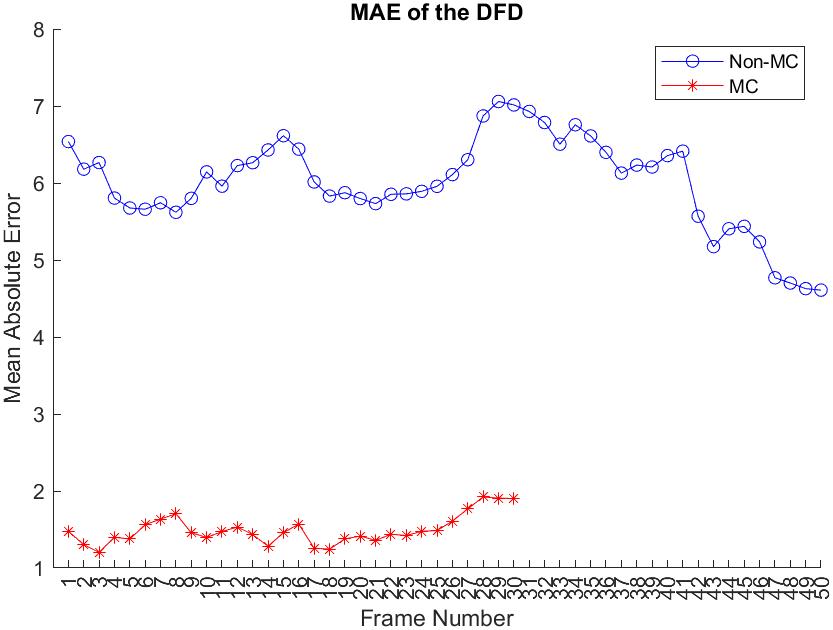
\includegraphics[width=1\textwidth]{MCERR.png}
    \centering
    \caption{Motion Compensated and Non Motion Compensated DFD}
\end{figure}

\section{Analysis}
\subsection{Q 3.1}

\begin{figure}[!h]
    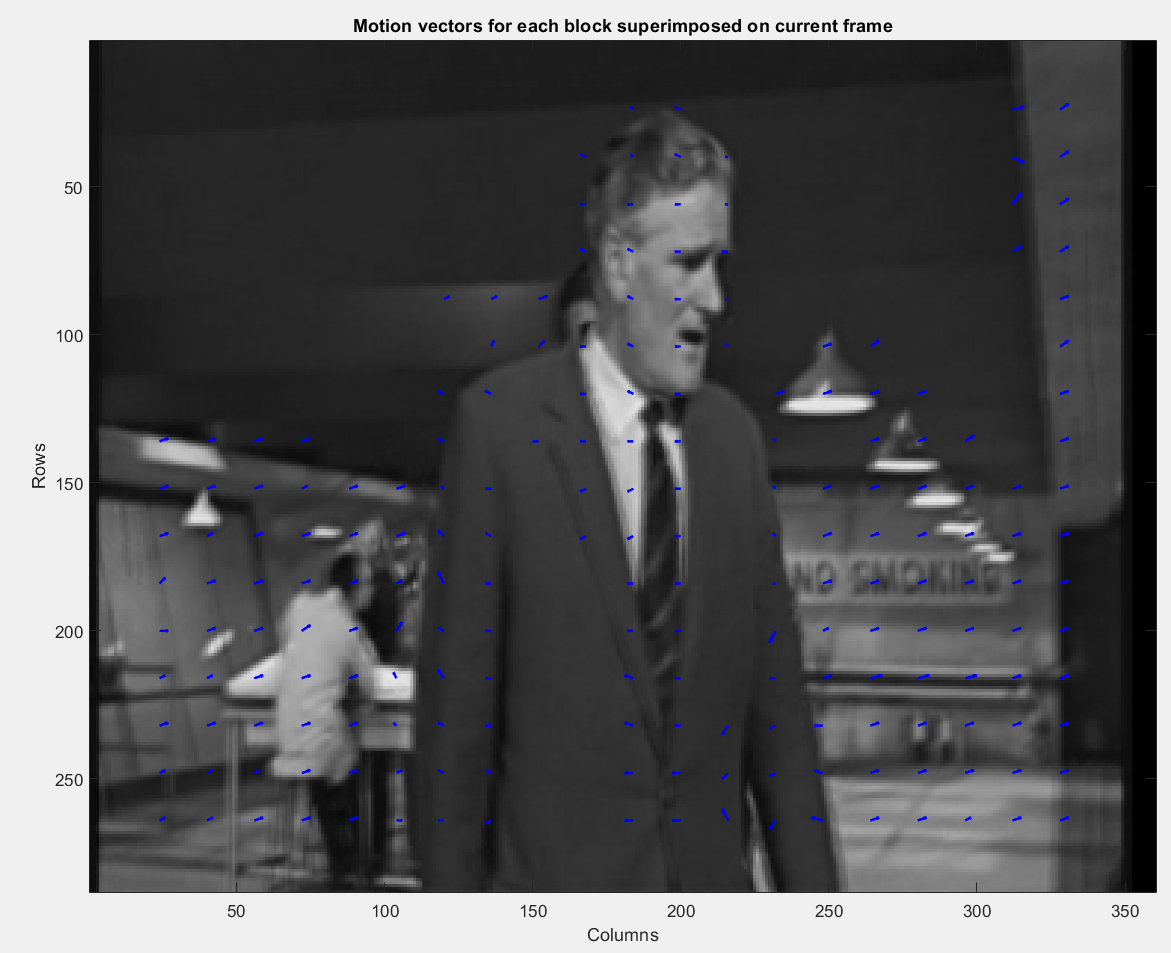
\includegraphics[width=1\textwidth]{frameN-2.png}
    \centering
    \label{fig:prevframe}
    \caption{Previous Frame}
\end{figure}

\begin{figure}[!h]
    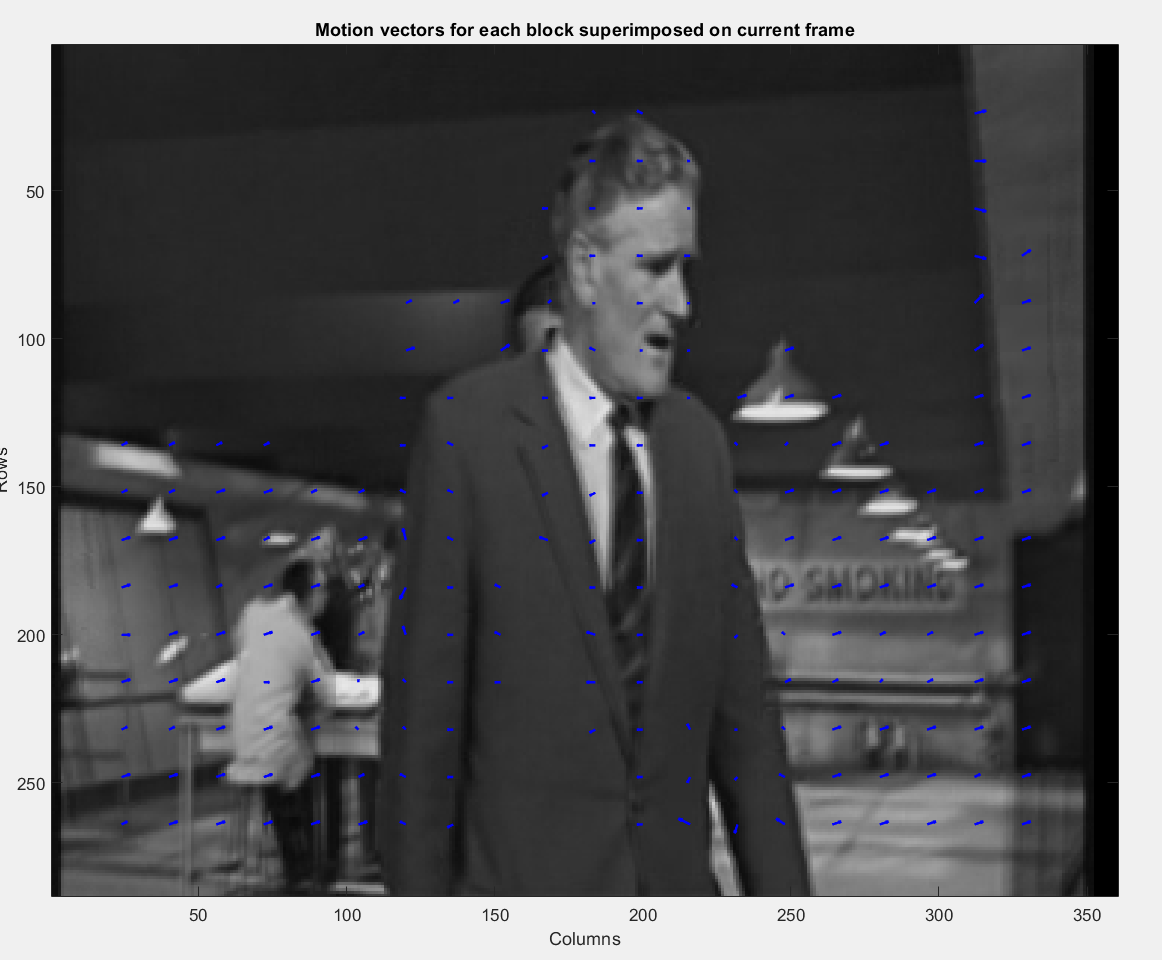
\includegraphics[width=1\textwidth]{frameN-1.png}
    \centering
    \caption{Current Frame}
\end{figure}

\begin{figure}[!h]
    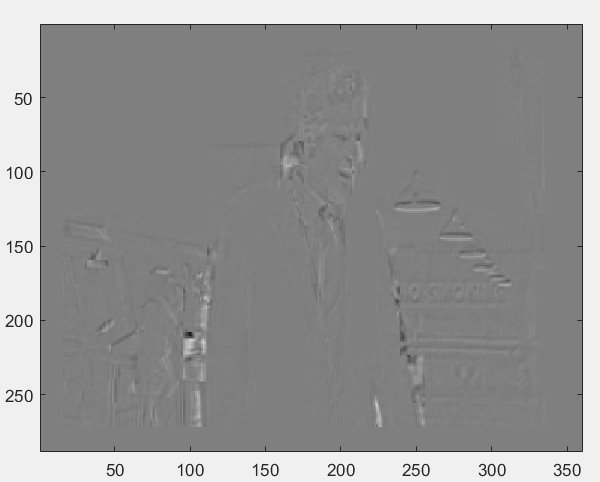
\includegraphics[width=1\textwidth]{frameN-2DFD.png}
    \centering
    \label{fig:prevframedfd}
    \caption{Previous Frame DFD}
\end{figure}


In the above two figures, we can see the motion vectors between the previous frame and the current frame. The motion
estimation works well in places that have a lot of texture, like the hair. The texturing of the hair provides a higher
chance of finding an accurate match between the previous frame and the current one. This is also evident when looking at
the DFD (Figure \ref{fig:prevframedfd}). In the region of the hair (250, 50), the DFD is very close to 0. One place that
the motion estimation fails slightly is in the areas of the suit. We know that the subject is moving to the right of the
frame and so we expect the suit that he is wearing to move as well. However in Figure \ref{fig:prevframe} we see that
there are no motion vectors in areas of the suit (150, 250). This could be because the suit isn't very textured, so the
block matching algorithm cannot detect any motion.

\subsection{Q 3.2}
For this section we had to vary the various parameters of the block matching algorithm such as the window search size,
the block size and the mae threshold and investigate their effects on the MAE. The following options were tried:

\begin{itemize}
    \item Motion Threshold: 1, Block Size: 04, Window Search Range: 2  
    \item Motion Threshold: 2, Block Size: 08, Window Search Range: 4   
    \item Motion Threshold: 3, Block Size: 16, Window Search Range: 8 
    \item Motion Threshold: 3, Block Size: 32, Window Search Range: 16
\end{itemize}

These provided the following MAEs:

\begin{itemize}
    \item MC-MAE: 1.798543, NMC-MAE: 5.942988, Time Taken: 1482.885735
    \item MC-MAE: 1.395298, NMC-MAE: 5.942988, Time Taken:  805.723205
    \item MC-MAE: 1.386106, NMC-MAE: 5.942988, Time Taken:  424.424478     
    \item MC-MAE: 1.449616, NMC-MAE: 5.942988, Time Taken:  707.205835
\end{itemize}

Notice how the MC-MAE, which corresponds to the MAE for the motion-compensated images, reduces as we increase the block
size and the window search range. This intuitively makes sense. Increasing the block size means that there is a higher
possibility of having unique features in that block that we can match to the previous frame. Increasing the window size
also helps in lowering the MAE since we provide the algorithm with more candidate locations for a match, increasing the
chance that we get a good match. However, increasing the window to be too large can cause the MAE to go up since the
algorithm could accidentally match it to a wrong block.

%% Motion Threshold: 1, Block Size: 04, Window Search Range: 02, MC-MAE: 1.798543, NMC-MAE: 5.942988, Time Taken: 1482.885735
%% Motion Threshold: 2, Block Size: 08, Window Search Range: 04, MC-MAE: 1.395298, NMC-MAE: 5.942988, Time Taken:805.723205
%% Motion Threshold: 3, Block Size: 16, Window Search Range: 08, MC-MAE: 1.386106, NMC-MAE: 5.942988, Time Taken: 424.424478
%% Motion Threshold: 3, Block Size: 32, Window Search Range: 16, MC-MAE: 1.449616, NMC-MAE: 5.942988, Time Taken: 707.205835
